\chapter{Detection of bank lines} \label{Chp3}

The location of bank lines is determined by looking at the transition of water to land (wet/dry) at a reference discharge computed using \dflowfm.
The detection of the bank lines builds on the search lines provided as input to this step.
The model domain is clipped to the area close to the search lines to focus the bank detection algorithm on the areas of interest only.
The exact location of the bank lines starts by determining for each grid cell in the area of interest whether it has one (or more) bed levels $z_b$ (defined at the mesh nodes) above the water level $z_w$ in the grid cell and one (or more) bed levels below the water level (see \autoref{Fig3.1}).

\Note \dfastbe currently only supports results of hydrodynamic simulations which use bed levels defined at nodes.
Simulations with bed levels defined in cells (tile depth) are thus not supported.

For each of those grid cells, the subgrid boundary between dry and wet parts is determined as the line along which the interpolated bed level equals the water level in the grid cell.
The line marking the zero water depth is a straight line in a triangle.
Cells with $N_c \ge 4$ corners are split in $N_c - 2$ triangles to arrive at a collection of only straight line segments.
The collection of all these line segments forms the basis of the final bank line.

\begin{figure}
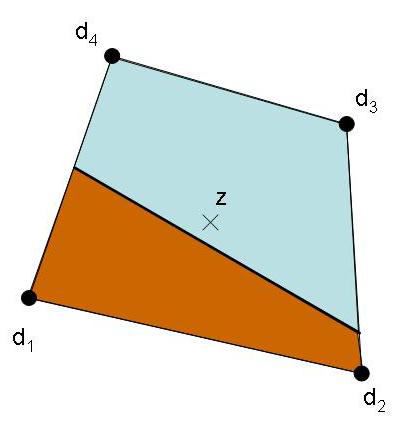
\includegraphics[width=5cm]{figures/Fig3-1.png}
\caption{Location of a bank line within a transition cell where $d$ equals $z_b$ and $z$ equals $z_w$}
\label{Fig3.1}
\end{figure}

The found locations of the bank lines will clearlu depend on the chosen discharge level.
However, as long as the discharge is within the main channel, the locations will be fairly consistent.

Generally, bank erosion only occurs along the main channel.
It is therefore possible to only take into account those cells that are within a certain distance from the predefined search lines.
This is also necessary when more than one bank line is present (as is common in rivers), because otherwise it is not clear which coordinates belong to one bank or the other.

For the Dutch rivers 'oeverlijnen' from Baseline can be used for these pre-defined lines.
These lines should be defined in a simple text file consisting of x- and y- coordinates (\command{Line1}, ..., \command{LineN}, in the configuration file).

One of the disadvantages of the 'oeverlijnen' from Baseline is that they only depict the main channel.
Possible side channels, shortcuts or lakes will then not be detected by the tool, see \autoref{Fig3.2}.
If they are important, extra lines should be added that (globally) represent the bank lines of these features.

\begin{figure}
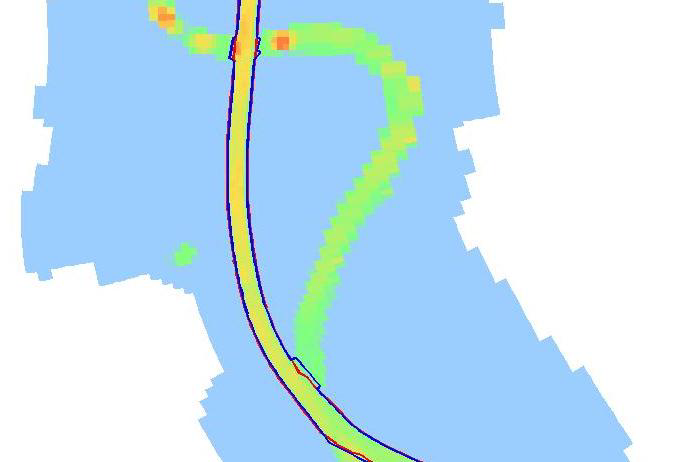
\includegraphics[width=\textwidth]{figures/Fig3-2.png}
\caption{Detection of bank lines at a shortcut in the Meuse river.
Red: Baseline 'oeverlijnen', Blue: detected bank line from WAQUA computation (Q = 278.5 m\textsuperscript{3}/s, average discharge)}
\label{Fig3.2}
\end{figure}

Groynes are not detected as such by the tool, because they are typically defined on subgrid level in the simulations, see \autoref{Fig3.3}.
The detected bank line is in this case following the banks within groyne sections.
This is an advantage, since possible bank erosion only takes place in the groyne sections and not along the groynes themselves.

\begin{figure}
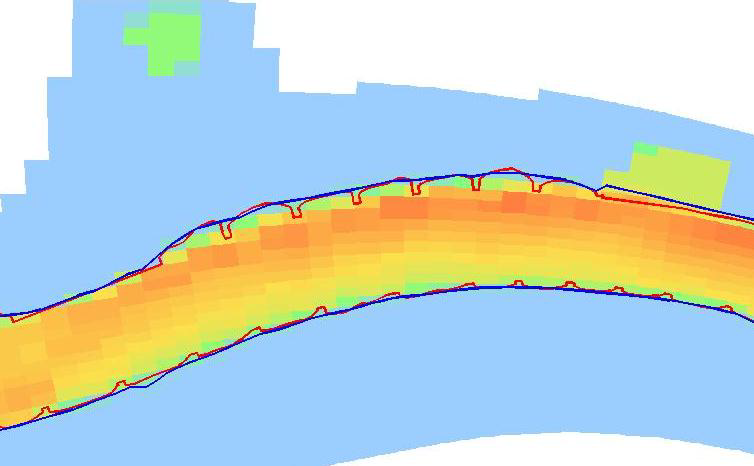
\includegraphics[width=\textwidth]{figures/Fig3-3.png}
\caption{Detection of a bank line close to groynes.
Red: Baseline 'oeverlijnen', Blue: detected bank line from WAQUA computation (Q=278,5 m\textsuperscript{3}/s, average discharge)}
\label{Fig3.3}
\end{figure}